\section{WASH}
While the schedulers we have examined already certainly have large improvements over existing schedulers, we could certainly do better.
On asymmetric processors a lot of assumptions that are made about how we schedule multithreaded programs are broken.
In particular we can look at the threads of a single program and find threads which have a higher priority to finish quickly and actually do something about them finishing more quickly.
The WASH scheduler keeps track of how many other threads are waiting on each thread to release its locks \cite{Jibaja:2016:PPA:2854038.2854047}.

\subsection{Implementation}
WASH is implemented as an extension to the JikesVM Java Virtual Machine.
This allows the scheduler much further insight into the operation of each thread than a kernal space scheduler has.
The drawback of this implementation is that WASH can only set the core priorities of each virtual machine thread, it cannot influence the threads of other processes on the system.
If the application that WASH is scheduling is the primary load on the system this is not an issue, but it shows the difficulty in generalizing this solution \cite{Jibaja:2016:PPA:2854038.2854047}.

\subsubsection{Psudocode}

\begin{algorithm}[H]
\caption{WASH}\label{euclid}
\begin{algorithmic}
	\Function{WASH}{$T_A,T_V,C_B,C_S,t$}
		\State $T_A$: Set of application threads
		\State $T_V$: Set of VM service threads, $T_A \cap T_V = \emptyset$
		\State $C_B$: Set of big cores
		\State $C_S$: Set of small cores, $C_B \cap C_S = \emptyset$
		\State $t$: Thread to schedule where $t \in T_A \cup T_V$
		\If{$|T_A| \leq |C_B|$}
			\If{$t \in T_A$}{ Set Affinity of t to $C_B$ }
			\Else{ Set Affinity of $t$ to $C_B \cup C_S$}
			\EndIf
			\ElsIf{$t \in T_A$}
				\If{$\forall \tau \in T_A (\text{Lock\%}(\tau) \le \text{Lock}_{\text{Thresh}})$}
				\State Set Affinity of $t$ to $C_B \cup C_S$
			\EndIf
		\EndIf
	\EndFunction
\end{algorithmic}
\end{algorithm}
\cite{Jibaja:2016:PPA:2854038.2854047}
\subsection{Performance}
WASH is not unique in it's maximal utilization of the most powerful core, where it gains its performance advantages is being able to keep more threads running on the less powerful cores at the same time.
As can be seen in figure \ref{fig:WASH_benchmarks}; WASH not only has better completion time than competing schedulers, but also better total energy usage.
This is a result of it's more effective utilization of all the cores, not just the high power cores. 
\begin{figure}[h]
	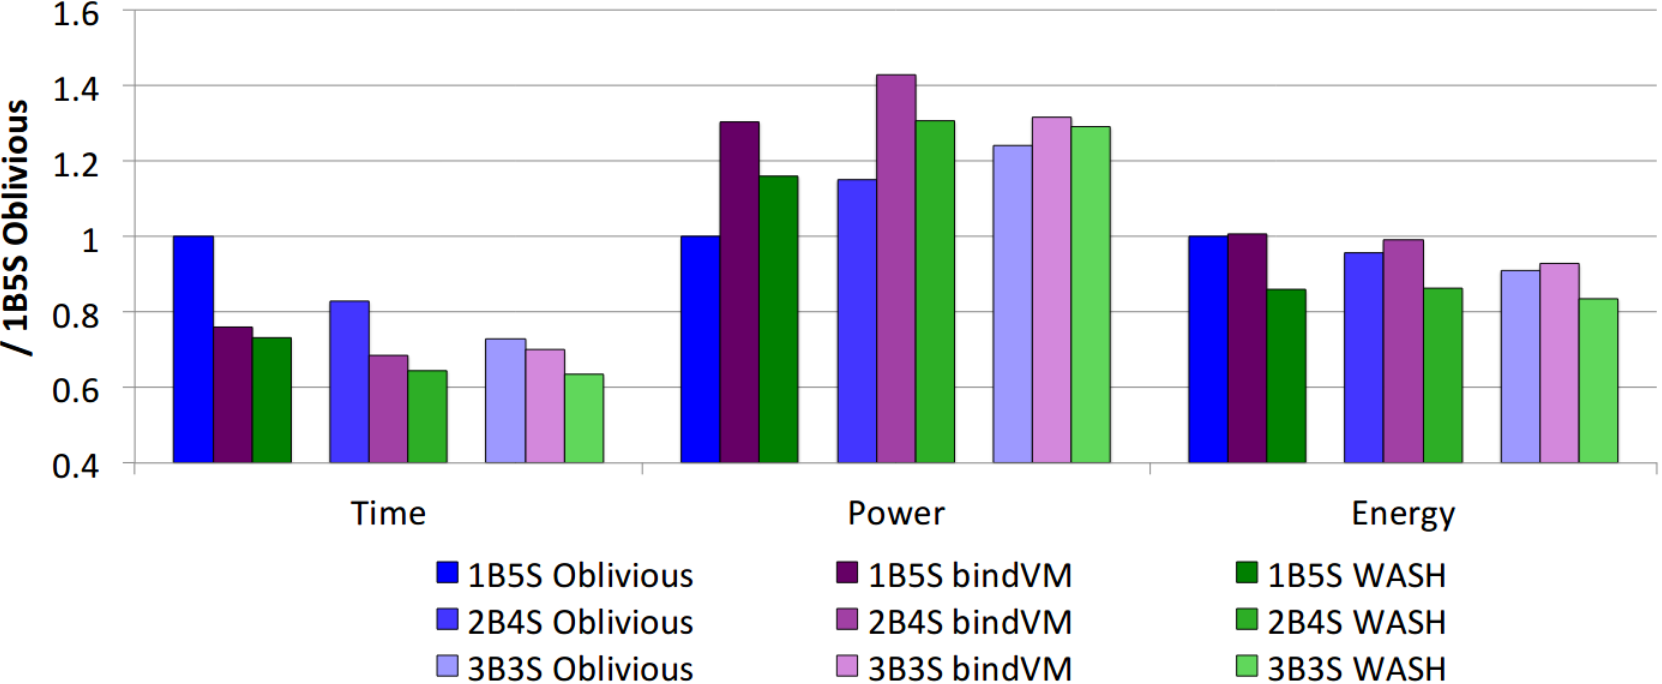
\includegraphics[width=\textwidth]{images/WASH_benchmarks.jpg}
	\caption{WASH compared to two other schedulers, default CFS (Oblivious), and helper threads manually bound to low power cores (bindVM), on three hardware configurations, 1B5S  (1Big core and 5 Small cores), 2B4S and 3B3S\cite{Jibaja:2016:PPA:2854038.2854047}.}
	\label{fig:WASH_benchmarks}
\end{figure}